%% Image Tikz pour le modèle à plusieurs états (Tx et Ty)


\tikzset{every picture/.style={line width=0.75pt}} %set default line width to 0.75pt        

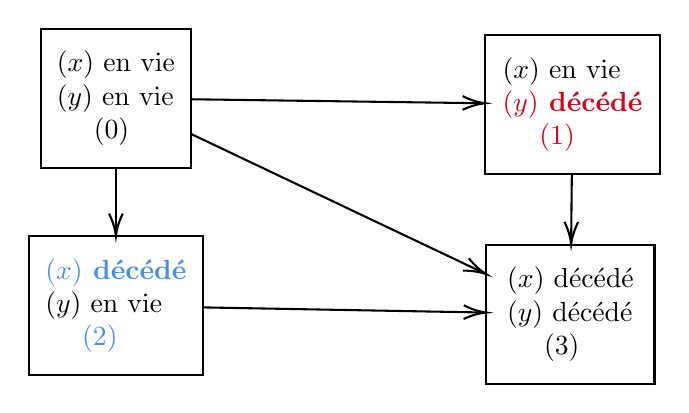
\begin{tikzpicture}[x=0.75pt,y=0.75pt,yscale=-1,xscale=1]
%uncomment if require: \path (0,300); %set diagram left start at 0, and has height of 300


% Text Node
\draw    (177,28.5) -- (249,28.5) -- (249,95.5) -- (177,95.5) -- cycle  ;
\draw (213,62) node  [align=left] {$\displaystyle ( x)$ en vie\\$\displaystyle ( y)$ en vie \\ \ \ \ \ $\displaystyle ( 0)$};
% Text Node
\draw    (391,31.5) -- (475,31.5) -- (475,98.5) -- (391,98.5) -- cycle  ;
\draw (433,65) node  [align=left] {$\displaystyle ( x)$ en vie \\\textcolor[rgb]{0.82,0.01,0.11}{$\displaystyle ( y)$\textbf{ décédé}} \\ \ \ \ \ \textcolor[rgb]{0.82,0.01,0.11}{$\displaystyle ( 1)$}};
% Text Node
\draw    (171,128.5) -- (255,128.5) -- (255,195.5) -- (171,195.5) -- cycle  ;
\draw (213,162) node  [align=left] {\textcolor[rgb]{0.29,0.56,0.89}{$\displaystyle ( x)$\textbf{ décédé}} \\$\displaystyle ( y)$ en vie \\ \ \ \ \ \textcolor[rgb]{0.29,0.56,0.89}{$\displaystyle ( 2)$}};
% Text Node
\draw    (391.5,132.5) -- (472.5,132.5) -- (472.5,199.5) -- (391.5,199.5) -- cycle  ;
\draw (432,166) node  [align=left] {$\displaystyle ( x)$ décédé \\$\displaystyle ( y)$ décédé \\ \ \ \ \ $\displaystyle ( 3)$};
% Connection
\draw    (249,62.49) -- (389,64.4) ;
\draw [shift={(391,64.43)}, rotate = 180.78] [color={rgb, 255:red, 0; green, 0; blue, 0 }  ][line width=0.75]    (10.93,-3.29) .. controls (6.95,-1.4) and (3.31,-0.3) .. (0,0) .. controls (3.31,0.3) and (6.95,1.4) .. (10.93,3.29)   ;

% Connection
\draw    (432.67,98.5) -- (432.35,130.5) ;
\draw [shift={(432.33,132.5)}, rotate = 270.57] [color={rgb, 255:red, 0; green, 0; blue, 0 }  ][line width=0.75]    (10.93,-3.29) .. controls (6.95,-1.4) and (3.31,-0.3) .. (0,0) .. controls (3.31,0.3) and (6.95,1.4) .. (10.93,3.29)   ;

% Connection
\draw    (249,79.1) -- (389.69,145.91) ;
\draw [shift={(391.5,146.77)}, rotate = 205.4] [color={rgb, 255:red, 0; green, 0; blue, 0 }  ][line width=0.75]    (10.93,-3.29) .. controls (6.95,-1.4) and (3.31,-0.3) .. (0,0) .. controls (3.31,0.3) and (6.95,1.4) .. (10.93,3.29)   ;

% Connection
\draw    (213,95.5) -- (213,126.5) ;
\draw [shift={(213,128.5)}, rotate = 270] [color={rgb, 255:red, 0; green, 0; blue, 0 }  ][line width=0.75]    (10.93,-3.29) .. controls (6.95,-1.4) and (3.31,-0.3) .. (0,0) .. controls (3.31,0.3) and (6.95,1.4) .. (10.93,3.29)   ;

% Connection
\draw    (255,162.77) -- (389.5,165.22) ;
\draw [shift={(391.5,165.26)}, rotate = 181.05] [color={rgb, 255:red, 0; green, 0; blue, 0 }  ][line width=0.75]    (10.93,-3.29) .. controls (6.95,-1.4) and (3.31,-0.3) .. (0,0) .. controls (3.31,0.3) and (6.95,1.4) .. (10.93,3.29)   ;


\end{tikzpicture}

